\documentclass[a4paper, 11pt]{article}

\usepackage{lmodern}
\usepackage{xcolor}
\usepackage[utf8]{inputenc}
\usepackage[T1]{fontenc}
\usepackage[francais]{babel}
\usepackage[top=1.7cm, bottom=1.7cm, left=2.5cm, right=2.5cm]{geometry}
\usepackage{verbatim}
\usepackage{tikz} %Vectoriel
\usepackage{listings}
\usepackage{fancyhdr}
\usepackage{multido}
\usepackage{amssymb}
\usepackage{multicol}
\usepackage{float}

\newcommand{\titre}{Réseau}
\newcommand{\numero}{5}
\newcommand{\typeDoc}{TDM}
\newcommand{\module}{Réseau}
\newcommand{\sigle}{reseau}
\newcommand{\semestre}{3}


\usepackage{ifthen}
\date{\today}

\rhead{Antoine de \bsc{Roquemaurel} (Groupe 1.1)}
\ifthenelse{\equal{\numero}{}}{
}
{
	\chead{\typeDoc~\no\numero}
}
\lhead{\titre}
%\makeindex

\lfoot{Université Toulouse III -- Paul Sabatier}
\rfoot{\sigle\semestre}
%\rfoot{}
\cfoot{--~~\thepage~~--}

\makeglossary
\makeatletter
\def\clap#1{\hbox to 0pt{\hss #1\hss}}%

\def\haut#1#2#3{%
	\hbox to \hsize{%
		\rlap{\vtop{\raggedright #1}
	}%
	\hss
	\clap{\vtop{\centering #2}
}%
\hss
\llap{\vtop{\raggedleft #3}}}}%
\def\bas#1#2#3{%
	\hbox to \hsize{%
		\rlap{\vbox{
			\raggedright #1
		}
	}%
	\hss \clap{\vbox{\centering #2}}%
	\hss
	\llap{\vbox{\raggedleft #3}}}
}%
\def\maketitle{%
	\thispagestyle{empty}{%
		\haut{}{\@blurb}{}
		%	
		%\vfill

		\begin{center}
			\vspace{-2.0cm}
			\usefont{OT1}{ptm}{m}{n}
			\huge \@type \@title
		\end{center}
		\par
		\vspace{7px}
		\hrule height 1pt
		\par
		\vspace{-0.8cm}
		\bas{}{}{}
}%
}
\def\date#1{\def\@date{#1}}
\def\author#1{\def\@author{#1}}
\def\type#1{\def\@type{#1}}
\def\title#1{\def\@title{#1}}
\def\location#1{\def\@location{#1}}
\def\blurb#1{\def\@blurb{#1}}
\date{\today}
\newboolean{monBool}
\setboolean{monBool}{true}
\author{}
\title{}
\ifthenelse{\equal{\numero}{}}{
	\type{\typeDoc~--- }
}
{
	\type{\typeDoc~\no\numero~--- }
}
\location{Amiens}\blurb{}
%\makeatother
\title{\titre}
\author{%Semestre \semestre
}

\location{Toulouse}
\blurb{%
\vspace{-35px}
\begin{flushleft}
	Université Toulouse III -- Paul Sabatier\\
	M1 Informatique -- Développement Logiciel\\
\end{flushleft}
\begin{flushright}
	\vspace{-55px}
	\large \textbf \module \\
	\normalsize \textit \today\\
	Semestre \semestre
	\vspace{30px}
\end{flushright}
Antoine de \bsc{Roquemaurel} (Groupe 1.1)
}%



%\title{Cours \\ \titre}
%\date{\today\\ Semestre \semestre}

%\lhead{Cours: \titre}
%\chead{}
%\rhead{\thepage}

%\lfoot{Université Paul Sabatier Toulouse III}
%\cfoot{\thepage}
%\rfoot{\sigle\semestre}

\pagestyle{fancy}

\definecolor{gris1}{gray}{0.40}
\definecolor{gris2}{gray}{0.55}
\definecolor{gris3}{gray}{0.65}
\definecolor{gris4}{gray}{0.50}
\definecolor{vert}{rgb}{0,0.4,0}
\definecolor{violet}{rgb}{0.65, 0.2, 0.65}
\definecolor{bleu1}{rgb}{0,0,0.8}
\definecolor{bleu2}{rgb}{0,0.2,0.6}
\definecolor{bleu3}{rgb}{0,0.2,0.2}
\definecolor{rouge}{HTML}{F93928}


\lstdefinelanguage{algo}{%
   morekeywords={%
    %%% couleur 1
		importer, programme, glossaire, fonction, procedure, constante, type, 
	%%% IMPORT & Co.
		si, sinon, alors, fin, tantque, debut, faire, lorsque, fin lorsque, 
		declenche, declencher, enregistrement, tableau, retourne, retourner, =, pour, a,
		/=, <, >, traite,exception, 
	%%% types 
		Entier, Reel, Booleen, Caractere, Réél, Booléen, Caractère,
	%%% types 
		entree, maj, sortie,entrée,
	%%% types 
		et, ou, non,
	},
  sensitive=true,
  morecomment=[l]{--},
  morestring=[b]',
}

\lstset{language=algo,
    %%% BOUCLE, TEST & Co.
      emph={importer, programme, glossaire, fonction, procedure, constante, type},
      emphstyle=\color{bleu2},
    %%% IMPORT & Co.  
	emph={[2]
		si, sinon, alors, fin , tantque, debut, faire, lorsque, fin lorsque, 
		declencher, retourner, et, ou, non,enregistrement, retourner, retourne, 
		tableau, /=, <, =, >, traite,exception, pour, a
	},
      emphstyle=[2]\color{bleu1},
    %%% FONCTIONS NUMERIQUES
      emph={[3]Entier, Reel, Booleen, Caractere, Booléen, Réél, Caractère},
      emphstyle=[3]\color{gris1},
    %%% FONCTIONS NUMERIQUES
      emph={[4]entree, maj, sortie, entrée},	
      emphstyle=[4]\color{gris1},
}
\lstdefinelanguage{wl}{%
   morekeywords={%
    %%% couleur 1
		importer, programme, glossaire, fonction, procedure, constante, type, 
	%%% IMPORT & Co.
		si, sinon, alors, fin, TANTQUE, tantque, FIN, PROCEDURE, debut, faire, lorsque, 
		fin lorsque, declenche, declencher, enregistrement, tableau, retourne, retourner, =, 
		/=, <, >, traite,exception, 
	%%% types 
		Entier, Reel, Booleen, Caractere, Réél, Booléen, Caractère,
	%%% types 
		entree, maj, sortie,entrée,
	%%% types 
		et, ou, non,
	},
  sensitive=true,
  morecomment=[l]{//},
  morestring=[b]',
}

\lstset{language=wl,
    %%% BOUCLE, TEST & Co.
      emph={importer, programme, glossaire, fonction, procedure, constante, type},
      emphstyle=\color{bleu2},
    %%% IMPORT & Co.  
	emph={[2]
		si, sinon, alors, fin , tantque, debut, faire, lorsque, fin lorsque, 
		declencher, retourner, et, ou, non,enregistrement, retourner, retourne, 
		tableau, /=, <, =, >, traite,exception
	},
      emphstyle=[2]\color{bleu1},
    %%% FONCTIONS NUMERIQUES
      emph={[3]Entier, Reel, Booleen, Caractere, Booléen, Réél, Caractère},
      emphstyle=[3]\color{gris1},
    %%% FONCTIONS NUMERIQUES
      emph={[4]entree, maj, sortie, entrée},	
      emphstyle=[4]\color{gris1},
}
\lstdefinelanguage{css}{%
   morekeywords={%
    %%% couleur 1
		background, image, repeat, position, index, color, border, font, 
		size, url, family, style, variant, weight, letter, spacing, line, 
		height, text, decoration, align, indent, transform, shadow, 
		background, image, repeat, position, index, color, border, font, 
		size, url, family, style, variant, weight, letter, spacing, line, 
		height, text, decoration, align, indent, transform, shadow, 
		vertical, align, white, space, word, spacing,attachment, width, 
		max, min, margin, padding, clip, direction, display, overflow,
		visibility, clear, float, top, right, bottom, left, list, type, 
		collapse, side, empty, cells, table, layout, cursor, marks, page, break,
		before, after, inside, orphans, windows, azimuth, after, before, cue, 
		elevation, pause, play, during, pitch, range, richness, spek, header, 
		numeral, punctuation, rate, stress, voice, volume,
	%%% types 
		left, right, bottom, top, none, center, solid, black, blue, red, green,
	},
  sensitive=true,
  sensitive=true,
  morecomment=[s]{/*}{*/},
  morestring=[b]',
}
\lstset{language=css,
    %%% BOUCLE, TEST & Co.
      emph={
		background, image, repeat, position, index, color, border, font, 
		size, url, family, style, variant, weight, letter, spacing, line, 
		height, text, decoration, align, indent, transform, shadow, 
		background, image, repeat, position, index, color, border, font, 
		size, url, family, style, variant, weight, letter, spacing, line, 
		height, text, decoration, align, indent, transform, shadow, 
		vertical, align, white, space, word, spacing,attachment, width, 
		max, min, margin, padding, clip, direction, display, overflow,
		visibility, clear, float, top, right, bottom, left, list, type, 
		collapse, side, empty, cells, table, layout, cursor, marks, page, break,
		before, after, inside, orphans, windows, azimuth, after, before, cue, 
		elevation, pause, play, during, pitch, range, richness, spek, header, 
		numeral, punctuation, rate, stress, voice, volume,
	  },
      emphstyle=\color{bleu2},
    %%% FONCTIONS NUMERIQUES
      emph={[3]
		left, right, bottom, top,none, solid, black, blue, green,
		  },
      emphstyle=[3]\color{bleu3},
    %%% FONCTIONS NUMERIQUES
}

\lstset{language=SQL,
    %%% BOUCLE, TEST & Co.
      emph={INSERT, UPDATE, DELETE, WHERE, SET, GROUP, BY, ORDER, REFERENCES},
      emphstyle=\color{bleu2},
    %%% IMPORT & Co.  
	emph={[2]
		if, end, begin, then, for, each, else, after, of, on, to
	},
      emphstyle=[2]\color{bleu1},
    %%% FONCTIONS NUMERIQUES
      emph={[3]Entier, Reel, Booleen, Caractere, Booléen, Réél, Caractère},
      emphstyle=[3]\color{gris1},
    %%% FONCTIONS NUMERIQUES
      emph={[4]entree, maj, sortie, entrée},	
      emphstyle=[4]\color{gris1},
}
\lstdefinelanguage{ARM}{%
   morekeywords={%
   ADD, SUB, MOV, MUL, RSB,CMP, BLS, BLE, B,BHI,LDR,
   BGE, RSBLT, BGT, BEQ, BNE,BLT,BHS,STR,STRB
	},
  sensitive=true,
  morecomment=[l]{@},
  morestring=[b]',
}

\lstset{ % general style for listings 
   numbers=left 
   , literate={é}{{\'e}}1 {è}{{\`e}}1 {à}{{\`a}}1 {ê}{{\^e}}1 {É}{{\'E}}1 {ô}{{\^o}}1 {€}{{\euro}}1{°}{{$^{\circ}$}}1 {ç}{ {c}}1 {ù}{u}1
	, extendedchars=\true
   , tabsize=2 
   , frame=l
   , framerule=1.1pt
   , linewidth=520px
   , breaklines=true 
   , basicstyle=\footnotesize\ttfamily 
   , numberstyle=\tiny\ttfamily 
   , framexleftmargin=0mm 
   , xleftmargin=0mm 
   , captionpos=b 
	, keywordstyle=\color{bleu2}
	, commentstyle=\color{vert}
	, stringstyle=\color{rouge}
	, showstringspaces=false
	, extendedchars=true
	, mathescape=true
} 
%	\lstlistoflistings
%	\addcontentsline{toc}{part}{List of code examples}
 %prise en charge du langage C 
\newcommand{\remarque}[1]{
	\begin{center}
	\medskip
	\colorbox{remarque}{
		\begin{minipage}{0.85\textwidth}\medskip
\includegraphics[height=10px]{images/remarque.png} #1 \medskip\end{minipage}
	}
	\medskip
	\end{center}
}

\newcounter{exemples}

\newenvironment{exemple}[1]{
   \vspace{-2mm}

\refstepcounter{exemples}
   \begin{center}
	\medskip
      \begin{minipage}{0.9\linewidth}
}{%
~
      \end{minipage}
   \end{center}~
   \vspace{-2mm}
}%

\newcommand{\captionExemple}[1]{
	\begin{center}{\bsc{Exemple} \thechapter.\arabic{exemples}~--~}#1\end{center}
}

\DeclareTextFontCommand{\policeGlossaire}{\fontfamily{lmss}\selectfont}
\DeclareTextFontCommand{\policePackage}{\fontfamily{phv}\selectfont}
\DeclareTextFontCommand{\policeTitre}{\fontfamily{ptm}\selectfont}
\newcommand{\policeCode}[1]{\texttt{#1}}

\newcommand{\sectionfont}{%
	\fontencoding{\encodingdefault}%
	\fontfamily{pag}%
	\fontseries{bc}%
	\fontshape{n}%
	\selectfont
}

% numéro du chapitre
\DeclareFixedFont{\chapnumfont}{T1}{phv}{b}{n}{80pt}
% pour le mot « Chapitre »
\DeclareFixedFont{\chapchapfont}{T1}{phv}{b}{n}{16pt}
% pour le titre
\DeclareFixedFont{\chaptitfont}{T1}{phv}{b}{n}{24.88pt}


\makeatletter
\def\thickhrulefill{\leavevmode \leaders \hrule height 1ex \hfill \kern \z@}
%% \chapter
\def\@makechapterhead#1{%
  \reset@font
  \parindent \z@
  \vspace*{10\p@}%
  \hbox{%
    \vbox{%
      \advance\hsize by -2cm
      \hrule height 0.4pt depth 0pt width \hsize
      \par
      \vskip 6pt%
      \hspace{20pt}%
      \parbox{420pt}{%
        \LARGE \bfseries #1
		}%
      \par
      \vskip 6pt%
      \hspace{20pt}%
      \hrule height 0.4pt depth 0pt width \hsize
	  \vspace{-30pt}
      }%
    \vbox{%
      \hsize=1.5cm%
      \begin{tabular}{c}
        \scshape \large \strut \@chapapp{} \\
        \colorbox{black}{\vbox{\hbox{\vbox to 1mm{}}\hbox{
			\color{white} \LARGE \bfseries \hspace{1mm}\thechapter\hspace{1mm}
		}\hbox{\vbox to 2cm{}}}}%
      \end{tabular}%
      }%
    }%
  \vskip 20\p@
}
%% \chapter*
\def\@makeschapterhead#1{%
  \reset@font
  \parindent \z@
  \vspace*{10\p@}%
  \hbox{%
    \vbox{%
      \advance\hsize by -0cm
      \hrule height 0.4pt depth 0pt width \hsize
      \par
      \vskip 6pt%
      \hspace{20pt}%
      \parbox{420pt}{%
        \LARGE \bfseries #1
		}%
      \par
      \vskip 6pt%
      \hspace{20pt}%
      \hrule height 0.4pt depth 0pt width \hsize
      }%
    }%
  \vskip 20\p@

}

\newlength{\sectiontitleindent}
\newlength{\subsectiontitleindent}
\newlength{\subsubsectiontitleindent}
\setlength{\sectiontitleindent}{-1cm}
\setlength{\subsectiontitleindent}{-.5cm}
\setlength{\subsubsectiontitleindent}{-.25cm}

\renewcommand{\section}{%
	\@startsection%
	{section}%
	{1}%
	{\sectiontitleindent}%
	{-3.5ex plus -1ex minus -.2ex}%
	{2.3ex plus.2ex}%
	{\sectionfont\Large}
}
\renewcommand{\subsection}{%
	\@startsection%
	{subsection}%
	{2}%
	{\subsectiontitleindent}%
	{-3.5ex plus -1ex minus -.2ex}%
	{2.3ex plus.2ex}%
	{\sectionfont\large}
}

\renewcommand{\subsubsection}{%
	\@startsection%
	{subsubsection}%
	{3}%
	{\subsubsectiontitleindent}%
	{-3.5ex plus -1ex minus -.2ex}%
	{2.3ex plus.2ex}%
	{\sectionfont\normalsize}
}

\makeatother




\makeatother
\newcommand{\http}{\bsc{http}}
\newcommand{\url}{\bsc{url}}
\newcommand{\ssh}{\bsc{ssh}}
\newcommand{\https}{\bsc{https}}
\newcommand{\osi}{\bsc{osi}}
\newcommand{\dns}{\bsc{dns}}
\newcommand{\udp}{\bsc{udp}}
\newcommand{\ip}{\bsc{ip}}
\newcommand{\tcp}{\bsc{tcp}}
\newcommand{\ftp}{\bsc{ftp}}
\newcommand{\mac}{\bsc{mac}}
\newcommand{\arp}{\bsc{ftp}}
\begin{document}
	\maketitle
	\section{Le concentrateur}
		\subsection{}
		\begin{figure}[H]
			\centering
			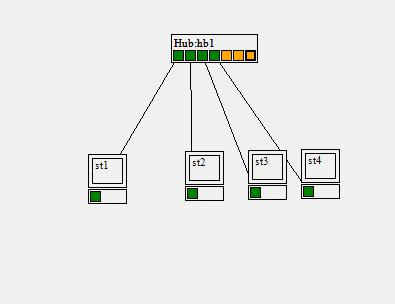
\includegraphics[width=8cm]{1.jpg}
			\caption{Création d'une topologie en étoile}
		\end{figure}
		\subsection{}
		\begin{description}
			\item[Unicast] Envoie d'un message à une seule machine du réseau
			\item[Broadcast] Envoie d'un message à toutes les machines du
				réseau\footnote{L'adresse de broadcast correspond au dernier bit, 255}.)
		\end{description}
		\subsection{}
		Non, st$_2$ et st$_4$ reçoivent également la trame.
		\subsection{}
		Un concentrateur envoie toujours tous les messages en broadcast, ce qui peut provoquer
		des collisions, cependant il n'a nullement connaissance de la position d'une machine.
%		Lorsque le concentrateur ne connait pas une machine sur le réseau, celui-ci va envoyer
%		une requête ARP à tout le réseau afin de trouver le bon destinataire. Une fois qu'il
%		connait la personne, il la notera dans une table Mac/port. Lors d'un envoie suivant,
%		si la station est présente dans la table mac port, le switch 
		\subsection{}
		Le concentrateur envoie bien la trame à tout le réseau, comme pour un envoie unicast,
		cependant cette fois-ci, toutes les stations sont destinataires, contrairement à un
		envoie unicast ou les stations n'interpretrons pas la trame, étant donné qu'elle ne
		les concernes pas.
	\section{Le commutateur}
	\subsection{}
		Le fonctionnement est correct.
	\subsection{}
	Dans les deux cas, seuls les destinataires reçoivent la trame, contrairement au
	concentrateur ci-dessus.
%	Si le cache ARP du commutateur est vidée, celui-ci ne peut situer les machines sur le
%	réseau, ainsi lorsqu'il envoie un paquet pour la première fois, il l'envoie en broadcast.
%	Ainsi dans le premier cas, tout le monde reçois la trame de ST$_3$ dans le deuxième cas,
%	tout le monde à l'exception de ST$_3$ reçoivent la trame.
	\subsection{}
	\'Etant donné que c'est une trame en broadcast, tout le monde reçois la trame.

	\subsection{}
	Un commutateur interprète les adresse \mac, lors d'un envoie d'un paquet, le switch
	vérifie dans sa table \mac port si le destinataire est présent, si c'est le cas il
	l'envoie sur le bon port, sinon il envoie en broadcast et met à jour la table\footnote{La
	nouvelle station, mais également les time to life}.
	\subsection{}
	le commutateur à mis à jour sa table mac port lors du premxier envoie, il est donc
	logique que la deuxième fois seul st$_4$ reçoit la trame.
	\subsection{}
	Tout le monde reçois la trame, en effet, le commutateur ne peut pas situer la machine sur
	le réseau. Une fois la trame reçus, celui-ci met sa table mac/port à jour.
	\subsection{}
	St$_1$, la table mac port à été mise à jour, il est capable de situer la machine sur le réseau.
	\subsection{}
	Seul ST$_4$ reçoit la trame, la table mac/port ayant été mise à jour, le switch est capable de situer la machine sur le
	réseau.
	\subsection{}
		\begin{figure}[H]
			\centering
			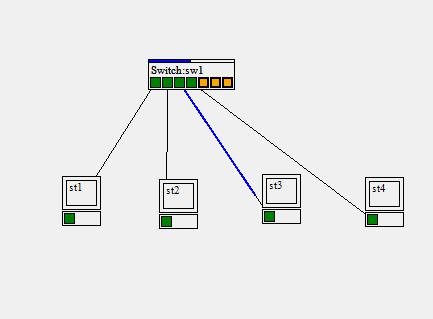
\includegraphics[width=8cm]{3.jpg}
			\caption{Test de réception}
		\end{figure}

	\section{Le routeur}
	\subsection{}
		\begin{figure}[H]
			\centering
			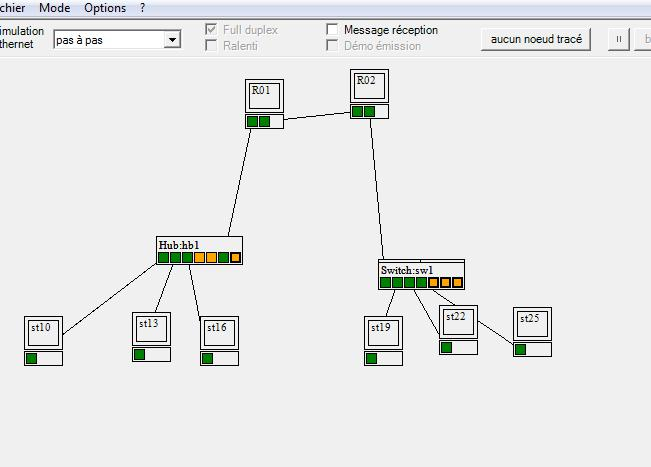
\includegraphics[width=8cm]{4.jpg}
			\caption{Conception}
		\end{figure}
	\subsection{}
	Non ils ne reçoivent pas la trame. Le routeur ne propage donc pas le domaine de diffusion,
	un routeur ne partage pas les messages de diffusions.
	\subsection{}
		\begin{figure}[H]
			\centering
			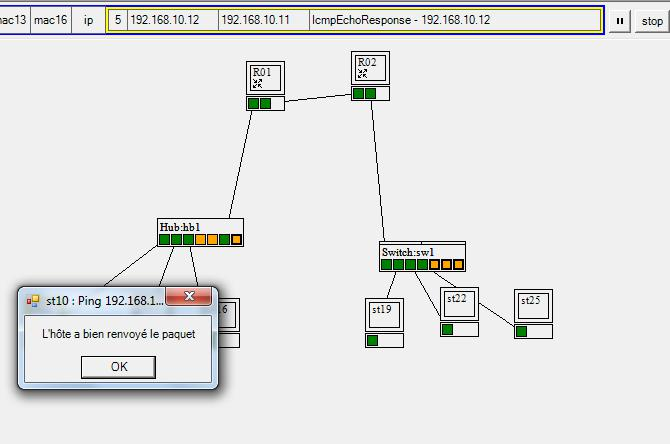
\includegraphics[width=7cm]{5.jpg}
			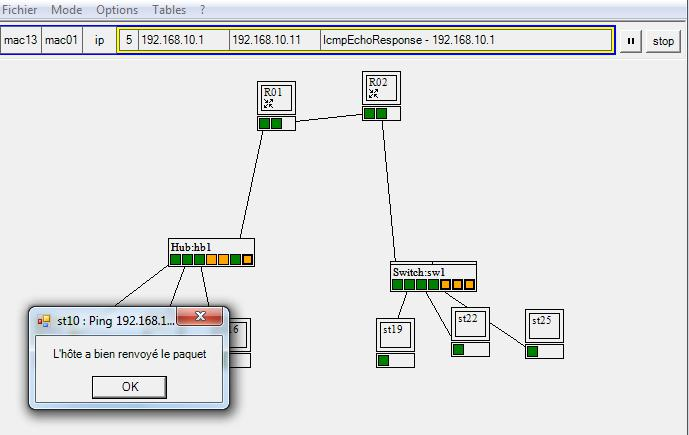
\includegraphics[width=7cm]{6.jpg}
			\caption{Ping}
		\end{figure}
		\subsection{}
		Impossible, étant donné qu'il ne trouve pas l'hôte. Ceci venant du fait qu'on a pas
		précisé ou se trouvais st$_5$ par rapport à st$_1$, c'est-à-dire sur un autre réseau.
		\subsection{}Oui, il y a un changement cette fois, le fil jaune, trace du ping, va
		jusqu'à R01 mais il affiche le message d'erreur <<Délai d'attente dépassé >>; En
		effet, la trame n'est pas capable de revenir.
		\subsection{}
		Oui, il y a tout d'abord une jonction via le commutateur, puis une fois la table de
		routage créée le ping passe. La trace jaune va maintenant sur l'autre routeur, donc la
		connexion entre les routeurs est bien effectuée, mais le délai d'attente est dépassé,
		cela prend trop de temps.
		\subsection{}
		Il faut rajouter à la station 5, l'adresse IP du routeur R02 dans l'interface, et il
		faut également rajouter une entrée vers R01 dans la table de routage R02, ainsi le
		paquet pourra revenir.
		\begin{figure}[H]
			\centering
			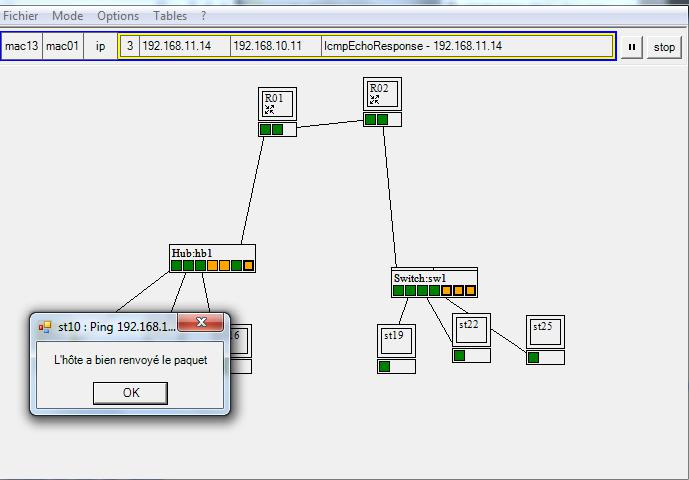
\includegraphics[width=8cm]{7.jpg}
			\caption{Test du ping réussis}
		\end{figure}
\end{document}
